%% ============================================================
%% 分片 21：原文第 8 节「Electric Eigenbranes」（原文 glshort.tex 起于第 6379 行）
%% 由 tools/harvmac2tex.py 从 arXiv 源码（hep-th/0604151v3）自动生成。
%% 只译英文散文；公式、编号、\label、\cite 一律不改。
%% ============================================================

\section{电特征膜}

\label{sec:electricbranes}

\begin{keytakeaways}
  \begin{itemize}[leftmargin=1.4em,itemsep=2pt,topsep=2pt]
    \item \textbf{物理图像}：Wilson 线算子作用于膜，就是把 Chan-Paton 丛（或层）与泛丛在 $p\in C$ 处的表示版本 ${\EUE}_p(R)$ 作张量积；由于 ${\EUE}_p(R)$ 一般只是扭化向量丛，这一作用同时把离散电场 ${\bf e}_0$ 平移 $\theta_R$。
    \item \textbf{数学工具}：零膜的 Chan-Paton 层是天穹层 $U_x$，限制到点上一切丛都平凡，于是特征值只是一个固定向量空间 ${\EUE}_q(R)|_x$；随 $q$ 变化它成为 $C$ 上平坦丛的纤维（取复结构 $J$ 时即泛平坦 $G_{\Bbb{C}}$ 丛），这正是几何 Langlands 一侧的数据。
    \item \textbf{关键结论}：支撑在 $\MH$ 光滑点 $x$ 的零膜是电特征膜；对它作 $S$-对偶得到 $\MH(G,C)$ 中支撑在 Hitchin 纤维 ${\CMF}$ 上、带秩一平坦 Chan-Paton 丛的磁特征膜（type ${\CMF}$ 膜），后者对应几何 Langlands 纲领中的 Hecke 特征层与完整 ${\cal D}$-模。
    \item \textbf{边界与展望}：更精确地说，电特征膜是不同 ${\bf e}_0$ 的扭化零膜之和，磁特征膜是 $\MH$ 各拓扑分支上膜之和；本文后续各节用 't Hooft 算子与 Hecke 算子的对应来验证 type ${\CMF}$ 膜确实具有 Hecke 特征层所需的性质。
  \end{itemize}
\end{keytakeaways}

在第~\ref{sec:loopop}~节中，我们引入了拓扑 Wilson 算子与 't Hooft 算子、它们对膜的作用，以及电特征膜与磁特征膜的概念。我们在第~\ref{sec:wilbranes}~节的目标是明确理解 Wilson 算子如何作用于膜。随后在第~\ref{sec:zerobelectric}~节，我们将利用这些信息把零膜辨认成电特征膜。

\subsection{Wilson 算子如何作用于膜}

\label{sec:wilbranes}

如本文一贯所述，所关心的理论是四维流形 $M$ 上规范群为 $G$ 的扭化 ${\cal N}=4$ 超 Yang-Mills 理论。场中包括 $G$-丛 $E\to M$ 上的一个联络 $A$。我们假定 $M$ 有一个边界，该边界由尊重拓扑对称性的膜 ${\cal B}$ 所标记；当然，这一条件依赖于参数 $\Psi$。

当 $\Psi=\infty$ 时存在拓扑 Wilson 线算子，我们通过取 $t=i$、规范耦合 $\tau$ 任意来实现这一点。设 $R$ 是 $G$ 的一个表示。表示 $R$ 中、支撑在曲线 ${\cal S}$ 上的 Wilson 算子在路径积分中贡献一个因子 % 式 (8.1)
\setcounter{equation}{0}
\begin{equation}\label{eq:yrgy}
W_{{\cal S}}(R)=P\exp\left(-\int_{{\cal S}}(A+i\phi)
 \right).
\end{equation}

更明确地说，记 $E(R)$ 为与 $E$ 相伴、在 $G$ 的表示 $R$ 中的丛。Wilson 线算子是在丛 $E(R)$ 中沿 ${\cal S}$ 的平行移动矩阵，所用联络为 $\CA=A+i\phi$。加入这个算子的效果是添加一个表示 $R$ 中的外源电荷，其在时空中的轨迹为 ${\cal S}$。若 ${\cal S}$ 是闭圈，我们取 $W_{{\cal S}}(R)$ 的迹；若 ${\cal S}$ 反而延伸到无穷远，则把 $W_{{\cal S}}(R)$ 与 ${\cal S}$ 两端的初态、末态结合起来，以得到规范不变的表达式。

现在特殊到 $M=\Sigma\times C$，以便把讨论约化为靶为 $\MH(G,C)$ 的二维 sigma 模型。
 在这个 sigma 模型中，${\cal B}$ 由靶空间 $\MH$ 上的一个 Chan-Paton 丛 $U$（也可能是更一般的层或层的复形 \cite{ref103,ref104}）表示。$U$ 带有一个联络 $\alpha$。既然膜 ${\cal B}$ 由它的 Chan-Paton 丛（或层）定义，Wilson 线算子就必须以某种方式作用于这个丛或层，从而作用于膜。

\begin{yizhu}[物理图像]
按：Wilson 线算子实际上就是带外源荷的平行移动矩阵；联络 $\CA=A+i\phi$ 中的 $i\phi$ 正是第~\ref{sec:topwil}~节为使 Wilson 线超对称而作的位移，闭圈情形取迹便得到规范不变的 Wilson 圈。它与式 \eqref{eq:tomfo} 的 Chan-Paton 边界因子形式相同，这正是下文把 Wilson 线的作用化为「与泛丛张量积」的出发点。
\end{yizhu}

让我们回顾 Chan-Paton 丛如何进入 sigma 模型。考虑映射 $\Phi:\Sigma\to \MH$ 的 sigma 模型，以及一个带有 Chan-Paton 丛 $U\to \MH$ 与联络 $\alpha$ 的膜 ${\cal B}$。量子理论由对可能映射 $\Phi$ 的积分定义，并伴随某些费米子变量。路径积分中的一个因子来自体作用量 ${\cmmib I}$，其形式为 $\exp\left(-\int_\Sigma {{\cmmib I}}\right)$。此外还有一个边界因子，涉及 Chan-Paton 丛中的平行移动。设 $\eurm Q$ 是 $\Sigma$ 的边界中由膜 ${\cal B}$ 标记的部分，并记 $\Phi_{\eurm Q}$ 为 $\Phi$ 到 $\eurm Q$ 的限制。路径积分中涉及 $\eurm Q$ 的边界因子由丛 $\Phi_{\eurm Q}^*(U)$ 沿 $\eurm Q$ 的平行移动或 holonomy 给出：
% 式 (8.2)
\setcounter{equation}{1}
\begin{equation}\label{eq:tomfo}
P\exp\left(-\int_{\eurm Q} \left(\Phi_{\eurm Q}^*(\alpha)
+\dots\right)\right).
\end{equation}
 若 $\eurm Q$ 是闭圈，我们取这个 holonomy 的迹；否则该因子在 $\eurm Q$ 的两端与其它因子结合——取决于所进行的具体计算——以给出规范不变的表达式。式 \eqref{eq:tomfo} 中的省略号是丛 $\Phi_{\eurm Q}^*(U)$ 上联络 $\Phi_{\eurm Q}^*(\alpha)$ 的费米子修正。超对称要求它们，正如第~\ref{sec:topwil}~节中为定义超对称 Wilson 算子需要平移 $A\to {\cal A}=A+i\phi$ 一样。

Chan-Paton 丛借以进入 sigma 模型的因子 \eqref{eq:tomfo} 与 Wilson 线算子借以影响底层四维规范场论的因子 \eqref{eq:yrgy} 之间有显然的类比。这个类比甚至更贴近，因为要定义 Wilson 算子对膜 ${\cal B}$ 的作用，我们必须取 ${\cal S}$（更确切地说，是它从 $\Sigma\times C$ 到 $\Sigma$ 的投影）逼近 $\eurm Q$ 的极限。

\begin{yizhu}[含糊点拨]
按：两个因子的类比要成为精确陈述，必须取「${\cal S}$ 的投影逼近 $\Sigma$ 的边界 $\eurm Q$」这一极限，此时 Wilson 线的围道与膜的边界重合。两式中的省略号（费米子项）都由拓扑对称性唯一确定，因此比较时不必逐项核对——这正是原文「不需要担心比较它们」的意思。
\end{yizhu}

为了从这个类比中得到确切的东西，我们从下面的观察开始。当 $G$-丛 $E\to M=\Sigma\times C$ 上的规范场论用映射 $\Phi:\Sigma\to \MH$ 描述时，$G$-丛 $E$ 可以等同于 $(\Phi\times 1)^*({\EUE})$，其中 ${\EUE}$ 是 $\MH$ 上泛 Higgs 丛 $({\EUE},\hat\varphi)$ 的「丛」部分，而 $(\Phi\times 1)^*({\EUE})$ 是它经由映射 $\Phi\times 1:\Sigma\times C\to \MH\times C$ 的拉回。这句话的意思只是：在 sigma 模型是良好描述的范围内，对每个点 $q\in \Sigma$，规范场论的玻色场 $A,\phi$ 限制到 $q\times C$ 上时，由对应于 $\Phi(q)\in \MH$ 的 Hitchin 方程解给出。这个解在相差一个规范变换的意义下正是泛 Higgs 丛 $({\EUE},\hat\varphi)$ 到 $\Phi(q)\times C$ 的限制。

为了用 sigma 模型解释 \eqref{eq:yrgy} 中的联络 ${\cal A}=A+i\phi$，我们注意到，一般地这个联络同时涉及 $\cA_\Sigma$（联络的切于 $\Sigma$ 的部分）与 $\cA_C$（切于 $C$ 的部分）。在低能理论中，我们可以假定 $\cA_C$ 服从 Hitchin 方程；并且只要避开 $\MH$ 的奇点，场 $\cA_\Sigma$ 在 sigma 模型中是有质量的。因此可以把它们积掉，换成 sigma 模型场 $\cA_C$。对非常大的 ${\rm Im}\,\tau$，在经典层次积掉 $\cA_\Sigma$ 就足够了。规范场论作用量中只依赖 $A$ 与 $\phi$ 的部分已在 \eqref{eq:wingo} 中写出。假定 $A_C$ 与 $\phi_C$ 满足 Hitchin 方程，并丢掉当 $C$ 的体积趋于零时消失的项，我们得到 $\cA_\Sigma$ 的二次作用量。相应的运动方程为
% 式 (8.3)
\setcounter{equation}{2}
\begin{equation}\label{eq:integrout}
\cD_C{}^\dagger \cD_C \cA_\Sigma=\cD_C{}^\dagger
d_\Sigma \cA_C+\dots,
\end{equation}
 其中 $\cD_C$ 是关于联络 $\cA_C$ 的协变微分。省略号指涉及四维规范场论费米子 $\psi$、$\tilde\psi$ 等的零模的项；我们不显式写出这些项。映射 $\Phi:\Sigma\to \MH$ 决定 $\cA_C$，从而也决定 $d_\Sigma \cA_C$；于是，假定远离 $\MH$ 的奇点，方程 \eqref{eq:integrout} 对 $\cA_\Sigma$ 有唯一解。

因此，一旦给定 $\Phi:\Sigma\to \MH$（并假定远离 $\MH$ 的奇点），联络 $\CA=(\cA_\Sigma,\cA_C)$ 就被确定。当然，$\CA$ 是丛 $E=(\Phi\times 1)^*({\EUE})$ 上的联络。实际上，$\CA$ 是 $\MH\times C$ 上丛 ${\EUE}\to \MH\times C$ 的某个联络 $\hat\CA$ 在 $\Phi\times 1$ 下的拉回。事实上，为定义 $\hat\CA$，必须指定它切于 $\MH$ 与 $C$ 的分量 $\CA_{\MH},\CA_C$。$\CA_C$ 是 Hitchin 方程的相应解，而 $\CA_{\MH}$ 由把 \eqref{eq:integrout} 以显然的方式推广来定义：\footnote{\eqref{eq:integrout} 中的省略号涉及费米子零模，它们代表 $\MH$ 的切向量，因而在 $\MH\times C$ 的情形中有类比物。}
% 式 (8.4)
\setcounter{equation}{3}
\begin{equation}\label{eq:pintegrout}
\cD_C{}^\dagger \cD_C \cA_{\M_H}=\cD_C{}^\dagger
d_{{\eusm M}_H} \cA_C+\dots.
\end{equation}

现在让我们特殊到 ${\cal S}=\gamma\times p$ 的情形，其中 $\gamma$ 是 $\Sigma$ 中的曲线、$p$ 是 $C$ 中的点。记 ${\EUE}_p(R)$ 为 ${\EUE}(R)$ 到 $\MH\times p$ 的限制。还记 $\Phi_p$ 为映射 $\Phi\times 1:\Sigma\times C\to \MH\times C$ 到 $\Sigma\times\{p\}\subset \Sigma\times C$ 的限制。我们可以把 \eqref{eq:yrgy} 中的联络 $\CA=A+i\phi$ 换成 $\Phi_p^*(\hat\CA)$。因此，路径积分中来自在围道 ${\cal S}$ 上、表示 $R$ 中插入 Wilson 算子的因子可以写成 % 式 (8.5)
\setcounter{equation}{4}
\begin{equation}\label{eq:zico}
W_R({{\cal S}})=
P\exp\left(-\int_\gamma\,\Phi_p^*(\hat\CA)\right).
\end{equation}
 当 $\gamma$ 逼近 $\Sigma$ 的边界 $\eurm Q$ 时，这与本来就从原膜 ${\cal B}$ 的 Chan-Paton 丛 $U$ 出现的项具有相同的形式：\footnote{式 \eqref{eq:zomfo} 中的省略号代表费米子项，它们在 \eqref{eq:zico} 中的类比物来自 \eqref{eq:integrout} 中的省略号，后者反映费米子对 $\CA_\Sigma$ 的贡献。所有这些项都由拓扑对称性唯一确定，因此不必费心比较它们。} % 式 (8.6)
\setcounter{equation}{5}
\begin{equation}\label{eq:zomfo}
P\exp\left(-\int_{\eurm Q} (\Phi_{\eurm Q}^*(\alpha)
+\dots)\right).
\end{equation}

于是我们得知 Wilson 线如何作用于膜。表示 $R$ 中、支撑在点 $p\in C$ 的 Wilson 线把膜 ${\cal B}$ 的 Chan-Paton 丛 $U$ 变换为 % 式 (8.7)
\setcounter{equation}{6}
\begin{equation}\label{eq:yuq}
U\to
U\otimes {\EUE}_p(R).
\end{equation}

\begin{yizhu}[物理图像]
按：式 \eqref{eq:yuq} 是本节的核心——Wilson 线在膜上的作用完全由泛丛在 $p$ 处的表示版本 ${\EUE}_p(R)$ 决定。但如紧接着的一段将说明的，${\EUE}_p(R)$ 一般只是扭化向量丛，所以这个张量积还会同时改变背景 $B$-场，亦即移动离散电场。这一点是后文 $S$-对偶论证的入口。
\end{yizhu}

\par\medskip\emph{$B$-场的变换}

如我们在第~\ref{sec:reviewthis}~节所讨论的，${\EUE}(R)$ 从而 ${\EUE}_p(R)$ 一般并不作为向量丛存在。但它总作为扭化向量丛存在，扭化为平坦 $B$-场 $\theta_{R}(\zeta)$，其中 $\theta_{R}$ 是由 $R$ 决定的规范群中心的特征标。

膜范畴依赖于 $B$-场的选取，这一事实我们在第~\ref{sec:comptwop}~节已加以利用。给定离散电场 ${\bf e}_0$，$\MH$ 上 sigma 模型中的背景 $B$-场为 $b_{{\bf e}_0}={\bf e}_0(\zeta)$，其中 $\zeta=\xi({\EUE}_{\rm{ad}})$ 是泛 $\bar G$ Higgs 丛存在的障碍。与扭化为 $\theta_R(\zeta)$ 的扭化丛作张量积，把扭化为平坦 $B$-场 $b$ 的膜映为扭化为 $b+\theta_R(\zeta)$ 的膜。因此，Wilson 线算子对膜的作用按 $b\to b+\theta_R(\zeta)$ 改变 $B$-场。换言之，它按 ${\bf e}_0\to {\bf e}_0+\theta_R$ 改变第~\ref{sec:centertop}~节所研究的离散电场。

我们想知道这个结果对 $S$-对偶意味着什么。于是把它写成关于对偶规范场论的陈述：对偶理论的规范群为 $^ LG$，Wilson 线 $W(^L\negthinspace R)$ 由表示 $^L\negthinspace R$ 决定。这条 Wilson 线按 % 式 (8.8)
\setcounter{equation}{7}
\begin{equation}\label{eq:nuko}
{\bf e}_0\to
{\bf e}_0+\theta(^L\negthinspace R),
\end{equation}
 变换离散电场，其中为方便起见，我们写 $\theta(^L\negthinspace R)$ 而不写 $\theta_{^L\negthinspace R}$。

\begin{figure}[htbp]
\centering
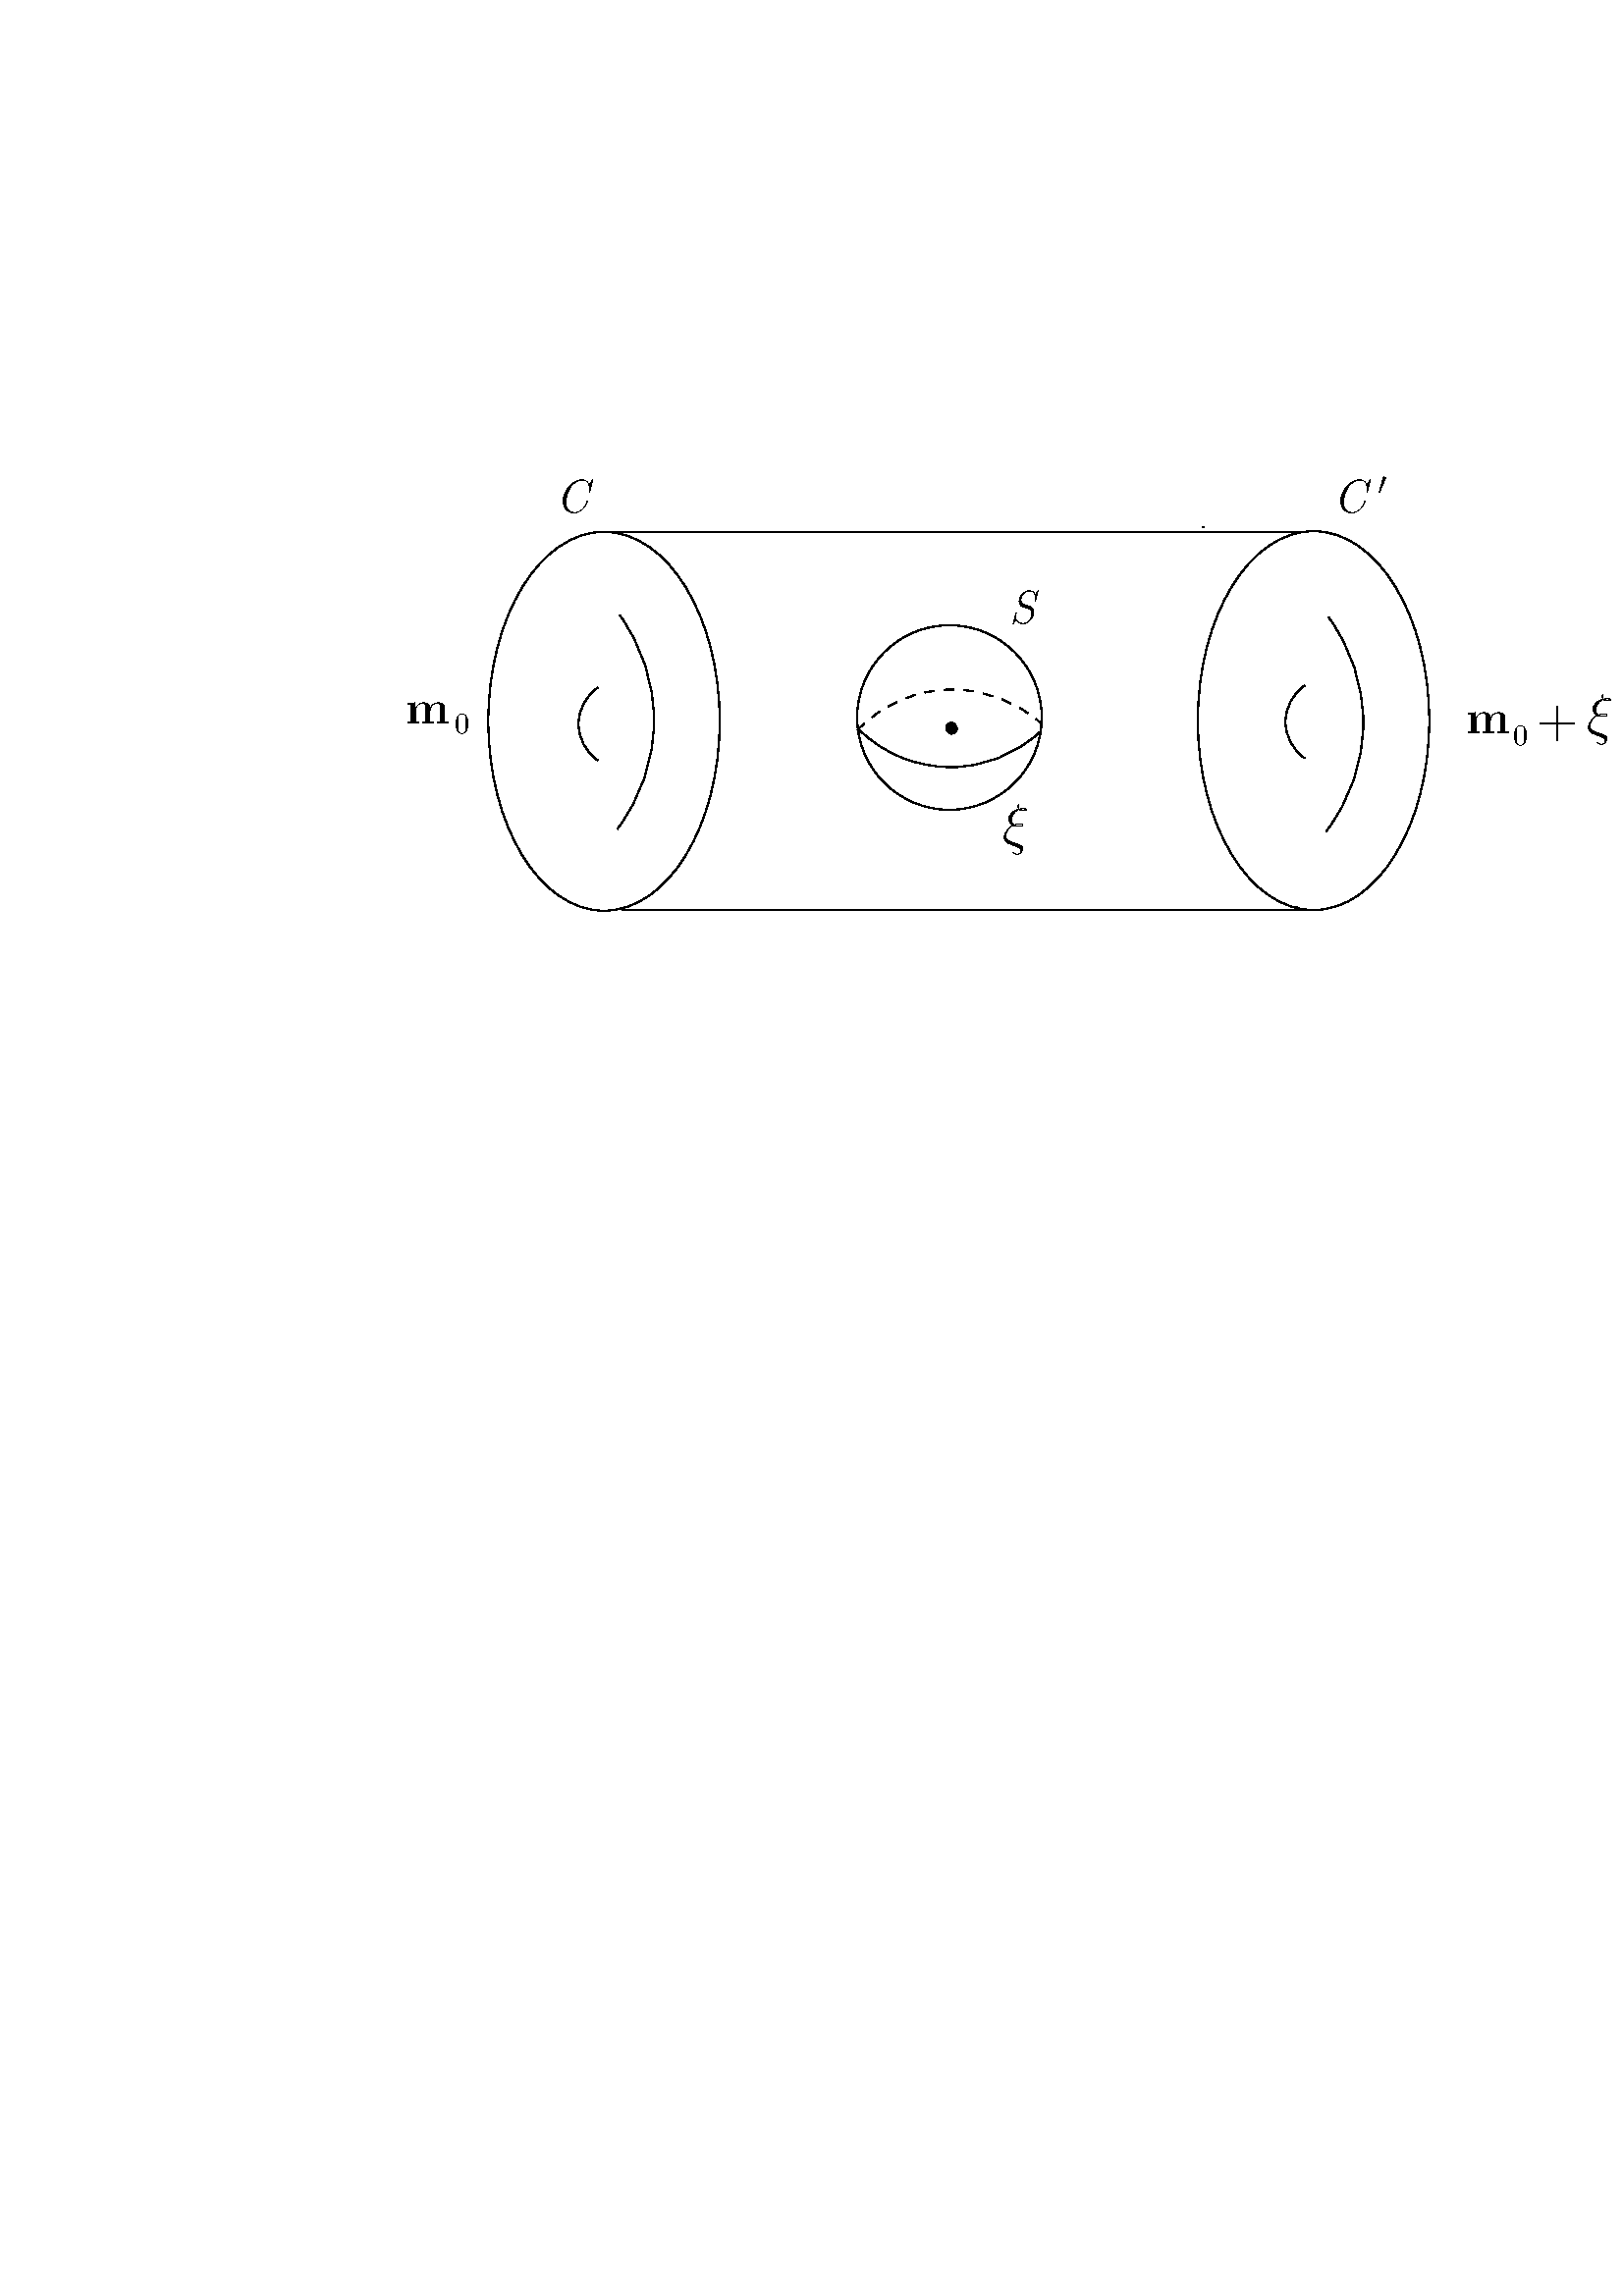
\includegraphics[width=0.75\linewidth]{figures/gla6-1.png}
\caption{插入一个 't Hooft 算子会改变 $G$-丛的拓扑，如图所示。图中画的是一个三维流形，其边界分支由两个黎曼面 $C$ 与 $C'$ 以及一个包围着 't Hooft 算子插入点的小二维球面 $S$ 组成。特征类的配边不变性意味着：若 ${\bf m}_0$ 是 $G$-丛 $E\to C$ 的特征类，则 $E\to C'$ 的特征类必为 ${\bf m}_0+\xi$，其中 $\xi=\xi({}^L\negthinspace R)$ 是与该 't Hooft 算子相联系的特征类。（原文 Fig.~11）}
\label{fig:namp}
\end{figure}
 在 $S$-对偶下，Wilson 线算子能改变离散电场 ${\bf e}_0$ 这一事实，对应着 't Hooft 线算子能改变特征类 ${\bf m}_0\in H^2(C,\pi_1(G))$ 这一事实，后者分类 $G$-丛 $E\to C$ 的拓扑。事实上，如我们在第~\ref{sec:tophooft}~节所解释的，'t Hooft 算子 $T(^L\negthinspace R)$ 是由 $S^2\cong \Bbb{CP}^1$ 上的一个 $G$-丛（可称之为 $E(^L\negthinspace R)$）构造的。这个 $G$-丛有特征类 $\xi(^L\negthinspace R)=\xi(E(^L\negthinspace R))$。't Hooft 算子对 ${\bf m}_0$ 的作用为 % 式 (8.9)
\setcounter{equation}{8}
\begin{equation}\label{eq:zuko}
{\bf m}_0\to {\bf
m}_0+\xi(^L\negthinspace R).
\end{equation}
 这个陈述是 \eqref{eq:nuko} 的 $S$-对偶，它只是来自特征类在配边下的行为，如 \namp 所示。

\begin{yizhu}[物理图像]
按：图 \ref{fig:namp} 的论证只用到特征类在配边下的不变性：三维流形的两个边界分支 $C$ 与 $C'$ 上 $G$-丛的特征类之差，等于包围 't Hooft 算子插入点的 $S^2$ 上 $G$-丛的特征类 $\xi$。这既给出式 \eqref{eq:zuko}，也解释了它为何是式 \eqref{eq:nuko} 在 $S$-对偶下的像。
\end{yizhu}

\par\medskip\emph{Wilson 算子与超对称}

让我们看看运算 \eqref{eq:yuq} 保持何种超对称。对曲线 ${\cal S}\subset \Sigma\times C$ 的一般选取，超对称 Wilson 线 $W(R,{\cal S})$ 只保持 $\MH$ 的复结构 $J$ 中的 $B$-型超对称，别的都不保持。然而，若取 ${\cal S}=\gamma\times p$，其中 $\gamma$ 是 $\Sigma$ 中的曲线、$p$ 是 $C$ 中的点，则 Wilson 算子保持更多超对称。事实上，正如我们在第~\ref{sec:lineop}~节末所证明的，它保持 $(B,B,B)$ 型超对称，即在每个复结构中都保持 $B$-型超对称。

现在我们能具体看出这一点如何反映在 Wilson 算子对膜的作用中。对点 $p\in C$，丛 ${\EUE}_p(R)$ 在 $\MH$ 的每个复结构下都是全纯的。（这可以用 $\MH$ 的超凯勒商构造自然地证明。）所以运算 \eqref{eq:yuq} 对每个复结构都保持 $B$-型超对称。

\subsection{零膜作为电特征膜}

\label{sec:zerobelectric}

现在我们可以寻找电特征膜了。考虑表示 $R$ 中、位于点 $q\in C$ 的 Wilson 线 $W_q(R)$。它把 Chan-Paton 层为 $U$ 的膜 ${\cal B}$ 映为 Chan-Paton 层为 $U\otimes {\EUE}_q(R)$ 的膜。按定义，若 $U\otimes {\EUE}_q(R)$ 与某个固定向量空间 $V$ 的 $U\otimes V$ 同构，则 ${\cal B}$ 是电特征膜。因此，条件就是：带有联络 $\Phi_q^*(\hat \CA)$ 的 ${\EUE}_q(R)$，当限制到 $U$ 的支撑集上时，必须是全纯平凡的——即同构于纤维为常数 $V$ 的向量丛。

设 $x$ 是 $\MH$ 中的一点，${\cal B}_x$ 是支撑在 $x$ 的零膜。换言之，${\cal B}_x$ 是 Chan-Paton 层为支撑在 $x$ 的天穹层 $U_x$ 的膜。我们将假定 $x$ 是 $\MH$ 的光滑点，从而可以在经典层次把场 $A_\Sigma,\phi_\Sigma$ 积掉。

任何向量丛限制到一点上都是平凡的，特别地丛 ${\EUE}_q(R)$ 限制到 $x\in \MH$ 上平凡。它到 $x$ 的限制（记作 ${\EUE}_q(R)|_x$）只是一个固定向量空间。所以
% 式 (8.10)
\setcounter{equation}{9}
\begin{equation}\label{eq:insto}
U_x\otimes {\EUE}_q(R)=U_x\otimes {\EUE}_q(R)|_x.
\end{equation}

因此，${\cal B}_x$ 是电特征膜，Wilson 圈算子 $W_q(R)$ 的「本征值」是向量空间 ${\EUE}_q(R)|_x$。

等价地，对应于零膜的 sigma 模型场边界条件说：$\cA_C$ 在 $\Sigma$ 的边界上在相差一个规范变换的意义下为常数。借助 \eqref{eq:integrout}，这意味着 ${\cal A}_\Sigma$ 在 $\Sigma$ 的边界上平凡。

我们在第~\ref{sec:lineop}~节基于底层四维拓扑场论论证过：电特征膜或磁特征膜的「本征值」必须随 $q\in C$ 变化，正如 $C$ 上平坦丛的纤维那样。确实，当 $q\in C$ 变化时，空间 ${\EUE}_q(R)|_x$ 正像平坦向量丛的纤维那样变化。事实上，取复结构 $J$，泛丛到 $x\times C$ 的限制 $({\EUE},\hat\varphi)|_x$ 给出平坦 $G_{\Bbb{C}}$ 丛 ${\EUE}|_x\to C$（因为 Hitchin 方程的解在复结构 $J$ 下对应平坦 $G_{\Bbb{C}}$-丛）。把这个丛取在表示 $R$ 中，就得到所需的平坦丛，其在 $q\in C$ 的纤维为 ${\EUE}_q(R)|_x$。我们这里选取复结构 $J$，是因为它被底层拓扑超对称特别挑出。

\begin{yizhu}[物理图像]
按：零膜的本征值虽然只是一个固定向量空间，但 $q$ 变化时它按 $C$ 上平坦丛的纤维变化；在复结构 $J$ 下这个平坦丛正是 Langlands 参数（平坦 $G_{\Bbb{C}}$ 丛）的表示版本。于是「电特征膜」同时承载了 Wilson 算子的本征值与一个局部系统——这正是几何 Langlands 对应中两侧数据会合的地方。
\end{yizhu}

在把零膜描述为电特征膜时，我们在一个关键点上稍显不正式：离散 $B$-场 ${\bf e}_0(\zeta)$ 的作用。$B$-场限制到一点上平凡，所以只要考虑零膜，就可以如我们刚才那样不正式地忽略 $B$-场。然而，更精确的描述方式如下。对每个 ${\bf e}_0$，膜范畴都包含一个对象，它是支撑在（光滑）点 $x\in \MH$ 的零膜。由于 Wilson 线算子的作用可以改变 ${\bf e}_0$，电特征膜实际上是具有不同 ${\bf e}_0$ 的扭化零膜之和（它们全都同构，因为扭化限制到一点上平凡）。对偶地，由于 't Hooft 算子可以改变 ${\bf m}_0$，磁特征膜将是支撑在 $\MH$ 不同分支上的膜之和，取遍所有可能的 ${\bf m}_0$。在几何 Langlands 纲领的标准处理中，人们说 Hecke 特征层支撑在 $\M(G,C)$ 的所有拓扑分支之并上。

\begin{yizhu}[易错点]
按：严格地说，电特征膜不是单个零膜，而是对每个 ${\bf e}_0$ 取一个在 $x$ 处的扭化零膜后作直和；这些扭化限制到点上都平凡，故彼此同构，但它们被 Wilson 算子相互联系（Wilson 算子把 ${\bf e}_0$ 平移）。对偶地，磁特征膜要对所有 ${\bf m}_0$ 分支求和，这正解释了为何 Hecke 特征层支撑在 $\M(G,C)$ 所有拓扑分支之并上，而不是单一分支上。
\end{yizhu}

\par\medskip\emph{与几何 Langlands 纲领的关系}

现在至少可以隐约看到这一切与几何 Langlands 纲领的关系。

在几何 Langlands 纲领中，人们从群 $^L\negthinspace G$ 以及同态 $\vartheta:\pi_1(C)\to{}^L\negthinspace G_{\Bbb{C}}$ 出发。（要求这个同态在第~\ref{sec:complexstr}~节所解释的某种意义下半稳定。）这样的同态构成的空间就是 Hitchin 模空间 $\MH(^L\negthinspace G,C)$。所以 $\vartheta$ 定义了 $\MH(^L\negthinspace G,C)$ 中的一点 $x(\vartheta)$。

若 $\vartheta$ 不可约，则 $x(\vartheta)$ 是光滑点，支撑在 $x(\vartheta)$ 的零膜 ${\cal B}_{x(\vartheta)}$ 是电特征膜。把 $S$-对偶作用于这个电特征膜，将得到靶为 $\MH(G,C)$ 的 sigma 模型中的磁特征膜。由第~\ref{sec:sdualhitfib}~节与第~\ref{sec:twodimint}~节可知，$\MH(^L\negthinspace G,C)$ 的零膜的 $S$-对偶是 $\MH(G,C)$ 中的膜，其支撑是 Hitchin 纤维化的一条纤维 ${\CMF}$，并配有秩一平坦 Chan-Paton 丛。我们把这样的膜称为 type ${\CMF}$ 的膜。

几何 Langlands 纲领的主要断言是：同态 $\vartheta:\pi_1(C)\to {}^L\negthinspace G_{\Bbb{C}}$ 以自然的方式联系着 $\M(G,C)$ 上的一个层，它既是 Hecke 特征层，又是完整的 ${\cal D}$-模。本文第~\ref{sec:thooftheckeop}~节至第~\ref{sec:abranes}~节将致力于解释为什么 $\MH(G,C)$ 上 type ${\CMF}$ 的膜具有正确的性质。在第~\ref{sec:thooftheckeop}~节与第~\ref{sec:bogeqheck}~节，我们把量子规范场论的 't Hooft 算子与几何 Langlands 纲领的 Hecke 算子联系起来，说明我们的磁特征膜概念如何与 Hecke 特征层的数学概念相关。在第~\ref{sec:abranes}~节，我们论证：由于 $\MH(G,C)$ 上存在某个余各向同性 $A$-膜，type ${\CMF}$ 的膜自然地联系着 $\M(G,C)$ 上微分算子的一个模。
